% !TeX root = Protokoll.tex
% !TeX root = ../../.global/latex/preamble.tex
\subsection{Aufbau}
\begin{figure}[h!]
		\centering
		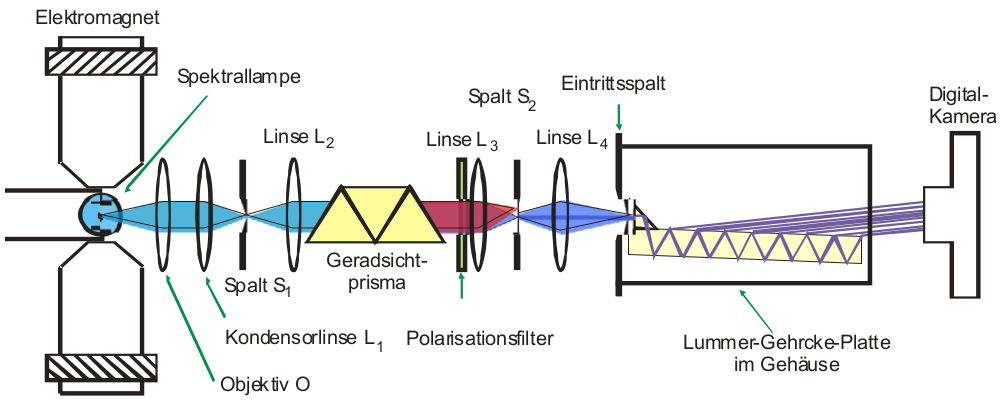
\includegraphics[width = 0.85\textwidth]{../Grafiken/Aufbau.jpg}
		\caption{Hier ist der Versuchsaufbau skizziert. \cite{V27}\label{fig:Versuchsaufbau}}
\end{figure}
\noindent
Der Verwendete Versuchsaufbau ist in \cref{fig:Versuchsaufbau} skizziert.
Die Cd-Lampe wird zwischen die Polschuhe eines Elektromagneten gebracht.
Das austretende Licht wird transversal zum Magnetfeld kollimiert und mithilfe
eines Glasprismas in seine Wellerlängen aufgeteilt. Durch einen Spalt kann eine dieser Wellenlängen ausgewählt werden.
Durch einen Polarisationsfilter kann die Spektrallinie auf $\pi$- oder $\sigma$-Übergänge untersucht werden.
Unter Zuhilfenahme einer Lummer-Gehrcke-Platte entsteht ein Interferenzmuster das mit einer Kamera photographiert wird.
Die Lumme-Gehrke-Platte erzeugt mithilfe von Interferenz ein hohes Auflösungsvermögen.
Damit sich zwei Wellenlängen nicht überlagern, darf deren Differenz nicht größer als das Dispersionsgebiet
\begin{align}
	\Delta \lambda_D =\frac{\lambda^2}{2d}\sqrt{\frac{1}{n^2-1}}
\end{align}
sein.
Dabei ist $d$ die Dicke der Platte und $n$ der Brechungsindex des Materials für die jeweilige Wellenlänge.
Das Auflösungsvermögen $A$, das mit dieser Platte erzielt werden kann ist durch
\begin{align}
	A=\frac{\lambda}{\Delta\lambda}=\frac{L}{\Lambda}(n^2-1)
\end{align}
bestimmt, dabei ist $L$ die Länge der Platte.
Die Eigenschaften der verwendeten Lummer-Gehrcke-Platte sind in \cref{tab:Lummer-Gehrcke} aufgeführt.
\begin{table}[h!]
	\centering
	\begin{tabular}{ccccc}
		\toprule
		Farbe & $\lambda/\si{\nano\meter}$& $n$ & $\Delta\lambda_D/\si{\nano\meter}$& $A$\\\midrule
		rot & $\num{643,8}$ & $\num{1,4567}$ & $\num{4.89e-2}$ & $\num{209e3}$\\
		blau & $\num{480,0}$& $\num{1,4635}$ & $\num{2,70e-2}$ & $\num{285e3}$\\\bottomrule
	\end{tabular}
	\caption{Hier sind die Parameter der Lummer-Gehrcke-Platte aufgeführt, wobei $d=\SI{4}{\milli\meter}$ und $L=\SI{120}{\milli\meter}$ sind. \label{tab:Lummer-Gehrcke}}
\end{table}
\newpage
\subsection{Messprogramm}
Zunächst wird das Magnetfeld für angelegte Ströme vermessen, um die Hysterese des Elektromagneten
zu bestimmen und das Magnetfeld zu eichen.
Anschließend wird die Lampe eingeschaltet und die Linsen werden justiert.
Die Messung beginnt mit dem $\sigma$-Übergang der roten Linie.
Dazu wird ein Foto der Spektrallinien ohne Magnetfeld gemacht.
Dann wird das Magnetfeld hochgefahren und es wird ein zweites Foto aufgenommen
zu dem Zeitpunkt an dem Sich die Linien soweit aufgeteilt haben, sodass sie
unterscheidbar sind, aber noch zu der ursprünglichen Linie zugeordnet werden können.
Diese Messung wird für die blaue Spektrallinie für die $\pi$- und $\sigma$-Übergänge wiederholt.
